\documentclass[tikz,border=10pt]{standalone}
\begin{document}
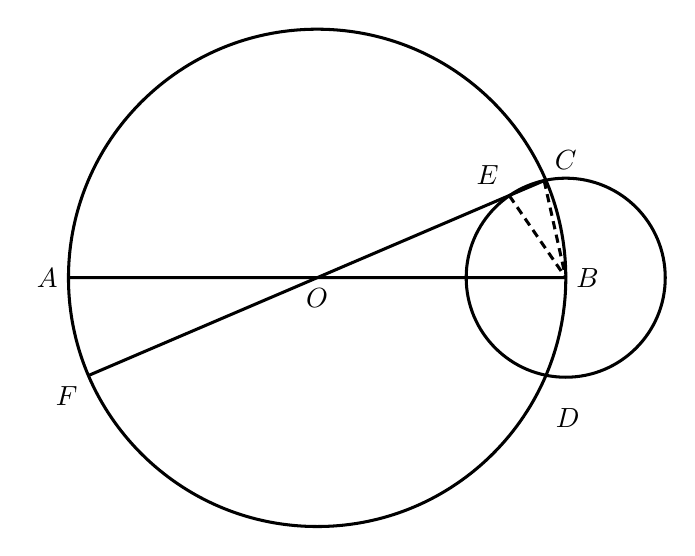
\begin{tikzpicture}[line width=1.1pt, line join=round]
% Coordinates in cm: s = 0.013378 cm/px, origin at ink-bbox centre (366,266 px), y flipped
\coordinate (A) at (-3.994,0.027);   % A (67.4,264)
\coordinate (O) at (-0.835,0.024);   % O (303.6,264.2), centre of big circle
\coordinate (B) at (2.322,0.026);    % B (539.6,264.0), centre of small circle
\coordinate (C) at (2.048,1.259);    % C (519.1,171.9)
\coordinate (E) at (1.606,1.067);    % E (486.1,186.2)
\coordinate (F) at (-3.741,-1.217);  % F (86.4,357.0)
\coordinate (D) at (2.060,-1.498);   % D (520,378), lower circle intersection

% Circles
\draw (O) circle[radius=3.158];      % big circle, R = 236 px
\draw (B) circle[radius=1.264];      % small circle, R = 94.5 px

% Solid diameter AB through O
\draw (A) -- (B);

% Solid slanted segment F-E-C
\draw (F) -- (C);

% Dashed segments E-B and C-B
\draw[dash pattern=on 3pt off 2pt] (E) -- (B);
\draw[dash pattern=on 3pt off 2pt] (C) -- (B);

% Labels
\node[left]        at (A) {\fontsize{10}{12}\selectfont $A$};
\node[right]       at (B) {\fontsize{10}{12}\selectfont $B$};
\node[above right] at (C) {\fontsize{10}{12}\selectfont $C$};
\node[below]       at (O) {\fontsize{10}{12}\selectfont $O$};
\node[above left]  at (E) {\fontsize{10}{12}\selectfont $E$};
\node[below left]  at (F) {\fontsize{10}{12}\selectfont $F$};
\node[below right] at (D) {\fontsize{10}{12}\selectfont $D$};
\end{tikzpicture}
\end{document}